\section{Debugger Testing DSL}

\emph{DeTeL} is open-source and is shipped as part of
mbeddr~\cite{mbeddrGithub}.
It is integrated in \ic{MPS} and interacts
with the mbeddr debugger \ic{API}. \emph{DeTeL} is currently tightly
coupled to mbeddr, however it could interact with a generic debugger \ic{API}
and could be implemented independent of \ac{MPS}.
This section describes the structure of \emph{DeTeL} and the
implementation of requirements discussed in \sect{DesignDecisions}. 
The language syntax is not documented, but can easily be derived by
looking at its editor definitions in \ac{MPS}. 

\subsection{DebuggerTest}
\label{DebuggerTestSection}

\fig{fig:DebuggerTestStructure} shows the structure of 
\ic{DebuggerTest}, which is a module that \emph{contains} 
\ic{IDebuggerTestContent}s, currently implemented by 
\ic{DebuggerTestcase} and \ic{CallStack} (described later). This interface
facilitates extensibility inside
\ic{DebuggerTest} (\hyperref[CS2]{CS2}). Further, \ic{DebuggerTest} refers to 
a \ic{Binary}, which is a concept from mbeddr representing the compiled mbeddr
program under test (\hyperref[R3]{R3}), 
the \emph{imports} of \ic{IDebuggerTestContent}s from
other \ic{DebuggerTest}s (\hyperref[CS1]{CS1}) and an
\ic{IDebuggerBackend} that specifies the debugger backend 
(\hyperref[CS2]{CS2}, \hyperref[MS1]{MS1}). The later is implemented by
\ic{GdbBackend} and allows this way to run debugger tests with the
\ac{GDB}~\cite{gdb}.

\vspace{1mm}
\begin{figure}[h]
  \vspace{-2mm}
  \centering
    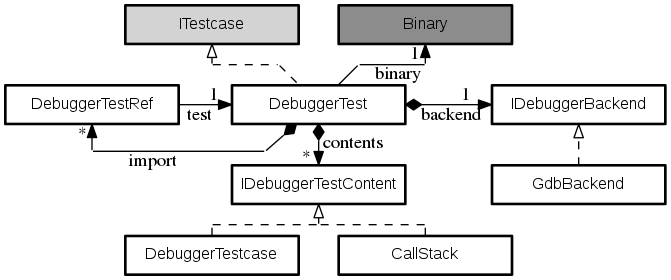
\includegraphics[width=8.8cm]{./figures/graph2-2.png} 
    \vspace{-3mm}
    \caption{Structure of \ic{DebuggerTest}}
  \label{fig:DebuggerTestStructure}
  \vspace{-2mm}
\end{figure}

\ac{MPS} already contains the language \ic{mps.lang.test} for writing type
system and editor tests. This allows (1) automatic execution
of tests on the command-line and 
(2) visualization of test results in a table view inside \ac{MPS}.
All of that functionality is built for future implementations of \ic{ITestcase}
- an interface from \ic{mps.lang.test}. By implementing this interface in
\ic{DebuggerTest} (our container for \ic{DebuggerTestcase}s), we benefit from
available features (\hyperref[CS3]{CS3}).

\subsection{CallStack}

\ic{CallStack} implements \ic{IDebuggerTestContent} 
(see \fig{fig:CallStackStructure}) and contains
\ic{IStackFrame}s (\hyperref[CS2]{CS2}, \hyperref[R1]{R1}),
which has two implementations:
\ic{StackFrame} and \ic{StackFrameExtension}.
An \emph{extend}ing \ic{CallStack} inherits all \ic{StackFrame}s
from the extended \ic{CallStack} in the form of \ic{StackFrameExtension}s, with
the possibility of specializing inherited properties (\hyperref[CS1]{CS1}), 
and can declare additional \ic{StackFrame}s.
\vspace{1mm}

\begin{figure}[h]
  \vspace{-3mm}
  \centering
    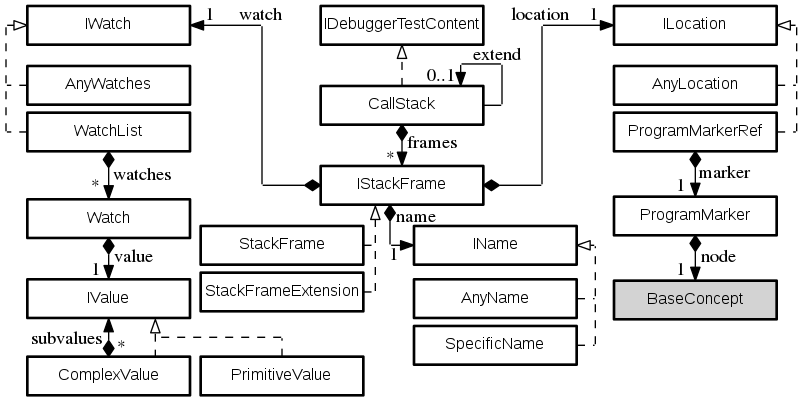
\includegraphics[width=8.8cm]{./figures/graph3-2.png} 
    \vspace{-2mm}
    \caption{Structure of \ic{CallStack}}
  \label{fig:CallStackStructure}
\end{figure}

\ic{IStackFrame} has three parts, each with two different implementations: a
\emph{name} (\ic{IName}), a location where program execution
should suspend (\ic{ILocation}) and visible \emph{watches}
(\ic{IWatch}es). 


\ic{IName} implementations: \ic{SpecificName} verifies
the specified \emph{name} matches the actual and \ic{AnyName} ignores it
completely. \ic{ILocation} implementations:
\ic{AnyLocation} that does not perform any validation and 
\ic{ProgramMarkerRef} that refers via \ic{ProgramMarker} to a specific
location in a program under test (\hyperref[R3]{R3}). These markers just
annotate nodes in the \ac{AST} and have no influence on code generation.
\ic{IWatch} implementations: \ic{AnyWatches} performs no validations and
\ic{WatchList} contains a list of \ic{Watch}es,
each specifies a \emph{name}/\emph{value} (\ic{IValue}) pair. The \emph{value}
can be either \ic{PrimitiveValue} (\eg numbers) or \ic{ComplexValue} (\eg arrays).

\subsection{DebuggerTestcase}

\fig{fig:DebuggerTestcaseStructure} shows the structure of
\ic{DebuggerTestcase}:
it can \emph{extend} other \ic{DebuggerTestcase}s (\hyperref[CS1]{CS1}),
has a \emph{name}, and can be \ic{abstract}. Further it contains the following
parts: \ic{SuspendConfig}, \ic{SteppingConfig} and
\ic{ValidationConfig}. Concrete \ic{DebuggerTestcase}s require  
a \ic{SuspendConfig} and a \ic{ValidationConfig} (can be inherited),
while an \ic{abstract} \ic{DebuggerTestcase} requires none of these.
 
\begin{figure}[h]
	\vspace{-3mm}
	\centering
    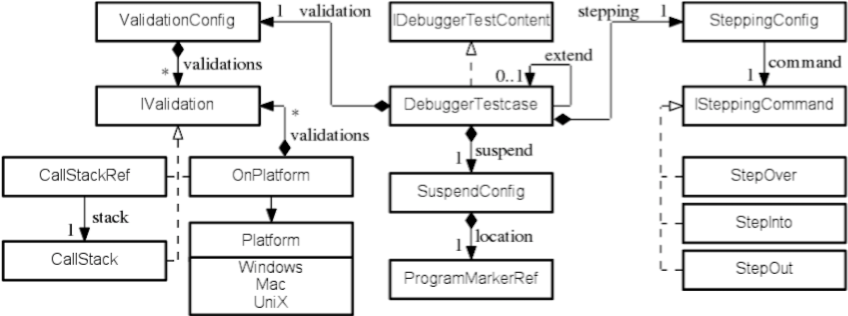
\includegraphics[width=8.7cm]{./figures/graph4_paper.png} 
    \vspace{-3mm}
	\caption{Structure of \ic{DebuggerTestcase}}
	\label{fig:DebuggerTestcaseStructure}
	\vspace{-2mm}
\end{figure}

\ic{SuspendConfig} contains a \ic{ProgramMarkerRef} that points to the first
program \emph{location} where execution suspends (\hyperref[R2]{R2}). 

\ic{SteppingConfig} is optional and contains a
list of \ic{IStep- pingCommand}s (\hyperref[CS2]{CS2}) that are executed after
suspending on \emph{location} (\hyperref[R2]{R2}). This interface is implemented by 
\ic{StepInto}, \ic{StepOver}, and \ic{StepOut} (each performs the
respective command n \emph{times}).

\ic{ValidationConfig} contains a list of \ic{IValidation}s
(\hyperref[CS2]{CS2}, \hyperref[R1]{R1}), implemented by
\ic{CallStack}, \ic{CallStackRef} and \ic{OnPlatform}.
\ic{CallStackRef} refers to a \ic{CallStack} that cannot
be modified. Finally, \ic{OnPlatform} specifies a \ic{Platform}
(\emph{Mac}, \emph{Unix} or \emph{Windows}) and contains \emph{validations},
which are only executed on the specific platform (\hyperref[R1]{R1}).

\section{Writing Debugger Tests}

In this section, we describe an application scenario where we apply \emph{DeTeL}  
to test the debugger extension of \ic{MUnit}. 

Before writing debugger tests, we first take the program using \ic{MUnit}
from \lst{lst:generatedUT} and annotate it in \lst{lst:annotatedProg}
with \ic{ProgramMarker}s. Those markers are later used by \ic{DebuggerTestcase}s 
for specification and verification of code locations where program
execution should suspend.

\begin{lstlisting}[language=markerDSL,caption=Annotated
program,label=lst:annotatedProg] 
int32 main(int32 argc, string$[$ $]$ argv) {
   [return test$[$forTest$]$;] onReturnInMain
}
int32 add(int32 a, int32 b) {
   [return a+b;] inAdd
}
testcase forTest {
   [int32 sum = 0;] onSumDeclaration
   [assert: sum == 0;] firstAssert
   [int32$[$ $]$ nums = {1, 2, 3};] onArrayDecl
   for(int32_t i=0;i<3;i++) { sum += nums[i]; }
   [assert: sum == 6;] secondAssert
}
\end{lstlisting}	

Next, in the \lst{lst:DebuggerTestingStub} a stub of \ic{DebuggerTest}
\emph{UnitTesting} is created that will later contain all \ic{DebuggerTestcase}s described in this
section. \emph{UnitTesting} tests against the \ic{Binary}
\emph{UnitTestingBinary}, which is compiled from \lst{lst:annotatedProg}.
Additionally, it instructs the debugger runtime to execute tests with the
\ic{GdbBackend}.

\begin{lstlisting}[language=testingDSL,caption=\ic{DebuggerTest} stub,
label=lst:DebuggerTestingStub]
DebuggerTest UnitTesting    tests binary: UnitTestingBinary {
                            uses debugger: gdb
}  
\end{lstlisting}

\subsection{Step Into ExecuteTestExpression}

For testing \emph{step into} on instances of \ic{Execute- TestExpression},
in the \lst{lst:callStacks}, we create a \ic{CallStack} that specifies
the stack organization after performing \emph{step
into} on \emph{onReturnInMain}. To reuse information and 
minimize redundancy in subsequent
\ic{DebuggerTestcase}s, two separate 
\ic{CallStack}s are created: First, \emph{csInMainFunction} 
contains a single \ic{StackFrame} that expects (1) program execution to suspend
at \emph{onReturnInMain} and (2) two \ic{Watch}es (\emph{argc} and
\emph{argv}). Second, \emph{csInTestcase} extends \emph{csInMainFunction} by adding an
additional \ic{StackFrame} \emph{forTest} on top of the \ic{StackFrameExtension}
\emph{main} (colored in gray). This \ic{StackFrame} specifies two \ic{Watch}es
(\emph{sum} and \emph{nums}) and no specific location
(\ic{AnyLocation}).

\begin{lstlisting}[language=testingDSL,caption=\ic{CallStack} declarations,
label=lst:callStacks]
call stack csInMainFunction {
   0:main
      location: onReturnInMain
      watches: {argc, argv}                     
}

call stack csInTestcase extends csInMainFunction {
   1:forTest
      location: <any>
      watches: {sum, nums}                  
   $\gT{0}$$\gT{:}$$\gT{main}$
}
\end{lstlisting}

\lst{lst:stepIntoTestcase} contains the \ic{DebuggerTestcase}
\emph{stepIntoTestcase}, which uses the \ic{CallStack} \emph{csInTestcase}
to verify \emph{step into} for instances of \ic{ExecuteTestExpression}. As
a first step, program execution is suspended at \emph{onReturnInMain}, next, a
single \ic{StepInto} is performed before the actual call stack is validated against
a custom \ic{CallStack} derived from \emph{csInTestcase}.
This custom declaration specializes the \ic{StackFrame}
\emph{forTest} \ie program execution is expected to suspend at
\emph{onSumDeclaration}.

\begin{lstlisting}[language=testingDSL,label=lst:stepIntoTestcase,
caption=\emph{Step into} \ic{ExecuteTestExpression}]
testcase stepIntoTestcase {            
   suspend at: 
      onReturnInMain
   then perform:                         
      step into 1 times    
   finally validate:                         
      call stack csOnSumDeclInTestcase extends csInTestcase {
         $\gT{1}$$\gT{:}$$\gT{forTest}$
            overwrite location: onSumDeclaration
            $\gT{watches}$$\gT{:}$ $\gT{\{}$$\gT{sum, nums}$$\gT{\}}$
         $\gT{0}$$\gT{:}$$\gT{main}$                       
      }
}
\end{lstlisting}
\vspace{-1mm}
\subsection{Step into/over AssertStatement}

After verifying \emph{step into} for
\ic{ExecuteTestExpression} in the previous section, we now test \emph{step into}
and \emph{over} for \ic{AssertStatement}. Both stepping commands have 
the same result when performed at
\emph{firstAssert}, hence common test behavior is extracted into the
\emph{abstract} \ic{DebuggerTestcase} \emph{stepOnAssert} as shown in
\lst{lst:AbstractDebuggerTest}: (1) program
execution suspends at \emph{firstAssert}, (2) a custom \ic{CallStack} verifies 
program execution suspended in \emph{forTest} on \emph{onArrayDecl} and
(3) the \ic{Watch} \emph{num} holds the \ic{PrimitiveValue} zero.
 
\begin{lstlisting}[language=testingDSL,caption=Abstract \ic{DebuggerTestcase},
label=lst:AbstractDebuggerTest]
abstract testcase stepOnAssert {
   suspend at: 
      firstAssert
   finally validate:
      call stack csOnArrayDeclInTestcase extends csInTestcase {
         1:forTest
            overwrite location: onArrayDecl
            overwrite watches: {sum=0,nums}
         0:main                      
      }
}
\end{lstlisting}

The \ic{DebuggerTestcase} \emph{stepIntoAssert} extending
\emph{stepOnAssert} performs a \ic{StepInto} command and \emph{stepOver- Assert}
performs a \ic{StepOver}:

\begin{lstlisting}[language=testingDSL,
caption=Extending \ic{DebuggerTestcase}s,label=lst:extendDTC] 
testcase stepIntoAssert extends stepOnAssert {            
   then perform:                         
      step into 1 times                            
}
testcase stepOverAssert extends stepOnAssert {            
   then perform:                         
      step over 1 times                            
}
\end{lstlisting}
\vspace{-1mm}
\subsection{Step on last Statement in Testcase}

The last testing scenario verifies that stepping on the last \ic{Statement}
(\emph{secondAssert}) inside a \ic{Testcase} suspends execution on the 
\ic{ExecuteTestExpression} (\emph{onReturnInMain}).
Again, we create an \emph{abstract} \ic{DebuggerTestcase}
\emph{steppingOnLastStmnt} that suspends
execution on \emph{secondAssert} and verifies that the actual call stack has the
same structure as \ic{CallStack} \emph{csInMainFunction}:

\begin{lstlisting}[language=testingDSL,
caption=Assumptions after suspending program execution in \emph{main}]
abstract testcase steppingOnLastStmnt {
   suspend at: 
      secondAssert
   finally validate:
      call stack csInMainFunction
}
\end{lstlisting}

Next, separate \ic{DebuggerTestcase}s are created, each for 
\emph{step over}, \emph{into} and \emph{out}, which extend
\emph{steppingOnLastStmnt} and specify only the respective \ic{ISteppingCommand}:

\begin{lstlisting}[language=testingDSL,
caption=Test stepping commands on last \ic{Statement} in \ic{Testcase}] 
testcase stepOverLastStmnt extends steppingOnLastStmnt { 
   then perform:                         
      step over 1 times                            
}

testcase stepIntoLastStmnt extends steppingOnLastStmnt {            
   then perform:                         
      step into 1 times                            
}

testcase stepOutFromLastStmnt extends steppingOnLastStmnt {            
   then perform:                         
      step out 1 times                            
}
\end{lstlisting}		

In each \ic{DebuggerTestcase} from the listing above execution suspends on the
same \ic{Statement} (\emph{OnReturnInMain}), although different stepping
commands are performed. Remember, since \emph{secondAssert} does not contain
any children of type \ic{StepIntoable} (\eg \ic{FunctionCall}), performing a
\emph{step into} on the \ic{Statement} has the same effect as
a \emph{step over}.

\section{Executing Debugger Tests}

Our test cases from the previous section are generated to plain Java code and
can be executed in \ac{MPS} with an action from the
context menu. This functionality is obtained by implementing \ic{ITestcase} in
\ic{DebuggerTest} (see \sect{DebuggerTestSection}).
By executing this action, test results are visualized in a table view, provided
by \ac{MPS}: for each \ic{DebuggerTestcase}, the result (success or
fail) is indicated with a colored bubble and a text field shows the
process output.

As indicated by a green bubble on the left side of \fig{fig:TestExecution1}, all
of our previously written \ic{DebuggerTestcase}s pass. 
We show in the next section how language evolution will invalidate the debugger
definition and this way cause all of our tests to fail.

\begin{figure}[h]
	\vspace{-2mm}
	\centering
    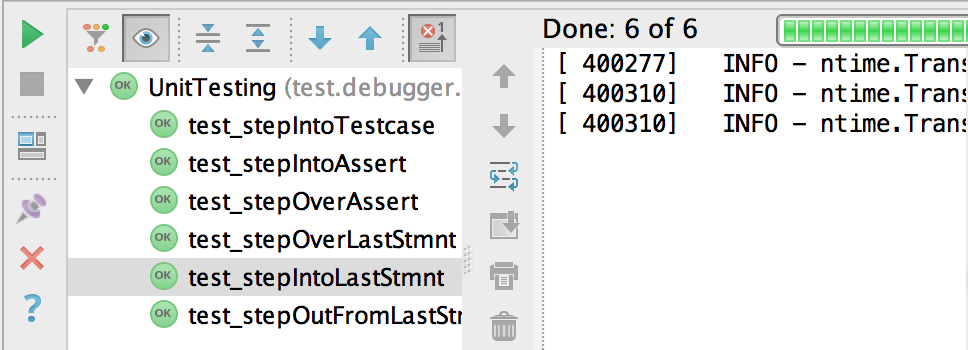
\includegraphics[width=8.4cm]{./figures/debuggerTestExec.png} 
    \vspace{-3mm}
	\caption{Successful execution of \ic{DebuggerTestcase}s in \ac{MPS}}
	\label{fig:TestExecution1}
	\vspace{-3mm}
\end{figure}